\documentclass{beamer}

\usepackage[utf8]{inputenc}
\usepackage{amssymb, amsfonts, latexsym, amsthm, amsmath, framed}
\usepackage{esvect}
\usepackage{parskip}

\usepackage{amsmath, amssymb, framed, tcolorbox}
\tcbuselibrary{theorems}

\usepackage{mathrsfs}
% \usepackage[hidelinks,colorlinks=true,linkcolor=blue,citecolor=blue]{hyperref}

\usepackage{xcolor}

\usepackage{natbib}
\bibliographystyle{plainnat}

\newcommand{\ba}{\backslash}
\newcommand{\Q}{\mathbb{Q}}
%\newcommand{\C}{\mathbb{C}}
\newcommand{\R}{\mathbb{R}}
\newcommand{\N}{\mathbb{N}}
\newcommand{\Z}{\mathbb{Z}}
\newcommand{\F}{\mathbb{F}}
\newcommand{\rank}{\text{rank}}

\newcounter{mytheorem}[section] \def\themytheorem{\thesection.\arabic{mytheorem}}

\definecolor{uva-orange}{RGB}{229, 114, 0}
\definecolor{uva-blue}{RGB}{35, 45, 75}
\definecolor{light-orange}{RGB}{249, 220, 191}
\definecolor{light-blue}{RGB}{200, 203, 210}
\tcbset{
theostyle/.style={fonttitle=\bfseries\upshape, colback=uva-orange!5,colframe=uva-orange!90},
defstyle/.style={fonttitle=\bfseries\upshape, colback=uva-blue!5,colframe=uva-blue!90},
corstyle/.style={fonttitle=\bfseries\upshape, colback=uva-blue!5,colframe=uva-blue!60!white},
exmstyle/.style={fonttitle=\bfseries\upshape, colback=uva-orange!5,colframe=uva-orange!60!white},
}
\tcbmaketheorem{defn}{Definition}{defstyle}{mytheorem}{def}
\tcbmaketheorem{theom}{Theorem}{theostyle}{mytheorem}{theo}
\tcbmaketheorem{coro}{Corollary}{corstyle}{mytheorem}{cor}
\tcbmaketheorem{exm}{Example}{exmstyle}{mytheorem}{eg}
\usecolortheme{custom}
\useoutertheme{infolines}
\useinnertheme{metropolis}
%%%%%%%%%%%%%%%%%%%%%%%%%%%%%%%%%%%%%%%%%%%%%%%%%%%%%%%%%%%%%
\title{Intrinsically Motivated Graph Exploration Using Network Theories of Human Curiosity}
%\subtitle{Modularity and Community Structure in Networks}
\date{Mar 21, 2024}
\author{Mia Yuan}
%\institute{DS8104}
%%%%%%%%%%%%%%%%%%%%%%%%%%%%%%%%%%%%%%%%%%%%%%%%%%%%%%%%%%%%%
\titlegraphic{\vspace{2cm}\flushright
\includegraphics[width=7cm,height=7cm]{uva.png}}
%%%%%%%%%%%%%%%%%%%%%%%%%%%%%%%%%%%%%%%%%%%%%%%%%%%%%%%%%%%%%
\begin{document}

%%%%%%%%%%%%%%%%%%%%%%%%%%%%%%%%%%%%%%%%%%%%%%%%%%%%%%%%%%%%%
\begin{frame}
\titlepage
\end{frame}

\AtBeginSection[]
{
	\begin{frame}{主要内容}
		\transfade%淡入淡出效果
		\tableofcontents[sectionstyle=show/shaded,subsectionstyle=show/shaded/hide]
		\addtocounter{framenumber}{-1}  %目录页不计算页码
	\end{frame}
}


%%%%%%%%%%%%%%%%%%%%%%%%%%%%%%%%%%%%%%%%%%%%%%%%%%%%%%%%%%%%%
\section{Human curiosity as graph exploration}
%%%%%%%%%%%%%%%%%%%%%%%%%%%%%%%%%%%%%%%%%%%%%%%%%%%%%%%%%%%%%

\begin{frame}{A brief introduction to Knowledge Graph}
\textcolor{red}{"... a graph of data intended to accumulate and convey knowledge of the real world, whose nodes represent entities of interest and whose edges represent potentially different relations between these entities."}
\begin{itemize}
    \item $\mathcal{V}$: Knowledge graphs represent relations between entities.
    \item $\mathcal{E}\subseteq \mathcal{V}\times \mathcal{V}$:Entities are nodes, and relationships are edges.
    \item Used for organizing complex sets of data.
\end{itemize}
\textbf{Tasks in KGs}
\begin{enumerate}
	\item Knowledge Representation Learning: Learn the representations.
	\item Knowledge Acquisition: Construct; Complete; Discover...
	\item Knowledge-Aware Application: NLP; Question answering; recommender system...
\end{enumerate}
\end{frame}
%%%%%%%%%%%%%%%%%%%%%%%%%%%%%%%%%%%%%%%%%%%%%%%%%%%%%%%%%%%%

\begin{frame}
\frametitle{Introduction}
\begin{center} 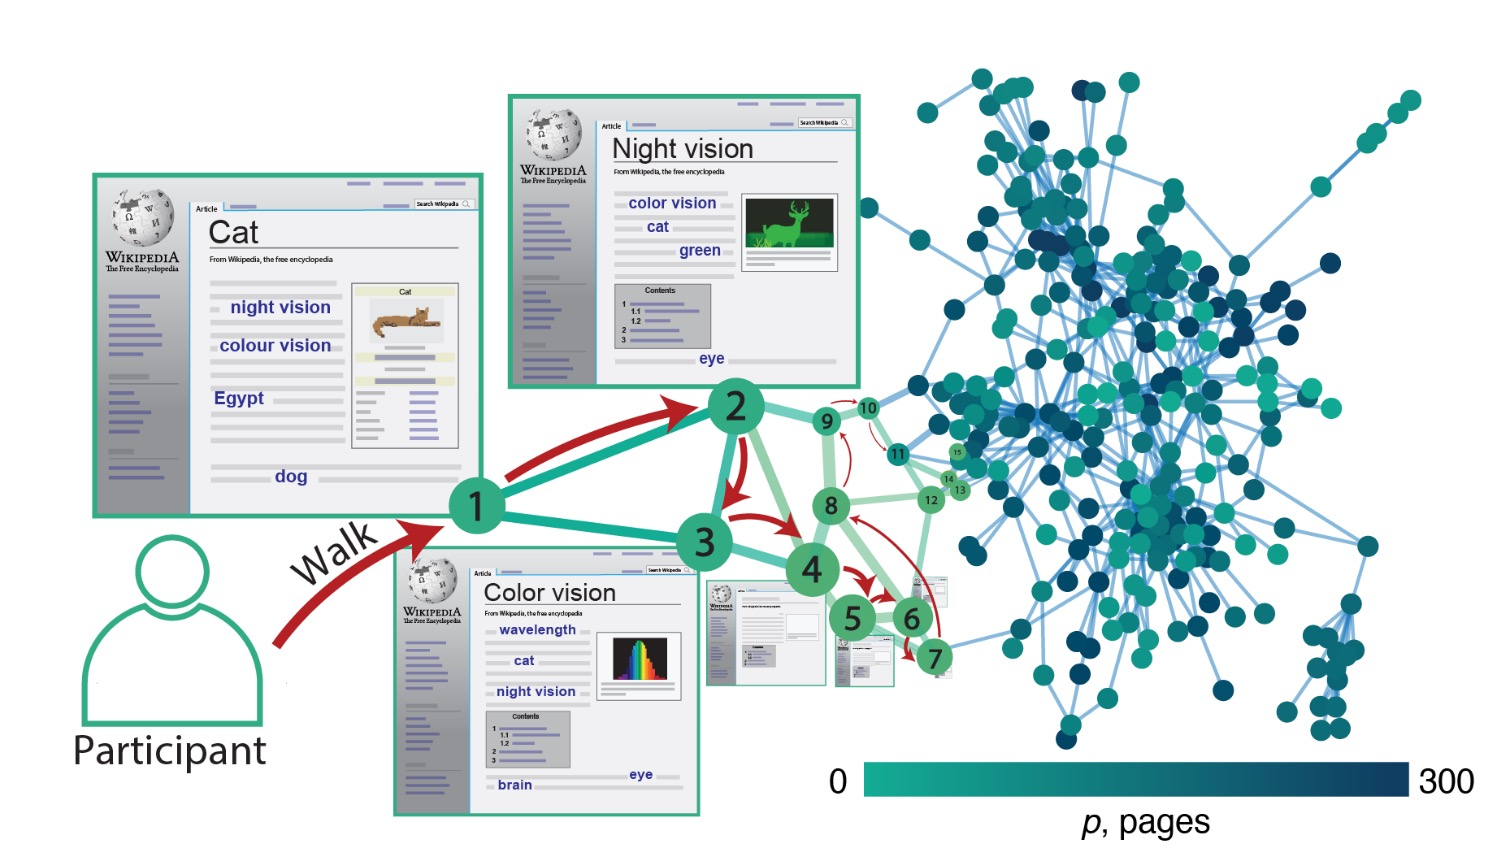
\includegraphics[scale=.35]{graph.jpg}\end{center}
\begin{enumerate}
    \item Task-agnostic?
    \item Human curiosity?
\end{enumerate}
\end{frame}

%%%%%%%%%%%%%%%%%%%%%%%%%%%%%%%%%%%%%%%%%%%%%%%%%%%%%%%%%%%%%

\begin{frame}{Curiosity -- Graph Exploration}
\textbf{Curiosity is the drive to acquire information that is missing from our understanding of the world.} 
\begin{enumerate}
\item Curiosity is an internally motivated search for information.
\item Think curiosity as a walk on a graph, given current time step $T$:
\begin{itemize}
\item The knowledge one already obtained -- the visited graph: $S_T$.
\item $\mathcal{V}_T=\lbrace v_1,...,v_T \rbrace \subseteq \mathcal{V}$: an ordered set of explored nodes at time $T$ -- explored knowledge.
\item Subgraph trajectory: $S_1 \subseteq S_2 \subseteq \cdots \subseteq S_T$.
\item Find an ordered set $\mathcal{V}^*_T$ to maximize total reward $\sum_{t=1}^T\gamma^{t-1}\mathcal{F}(S_t)$

\end{itemize}
\end{enumerate}

\end{frame}
%%%%%%%%%%%%%%%%%%%%%%%%%%%%%%%%%%%%%%%%%%%%%%%%%%%%%%%%%%%%%
\section{What drives curiosity?}
\begin{frame}{What is curiosity? -- Information Gap Theory}
People may obtain information purely to satisfy curiosity. Loewenstein (1994) proposed an information-gap account of curiosity, which provides insight about its situational determinants.\\
There are many things that people don’t know and that don’t bother them, but awareness of specific pieces of missing information can prompt an unreasonably strong desire to fill these gaps.
\begin{enumerate}
	\item Perception of a gap in one’s knowledge of the world creates an aversive state of uncertainty.
	\item Curiosity motivates a search for information to close the gap.
\end{enumerate}
\begin{center} 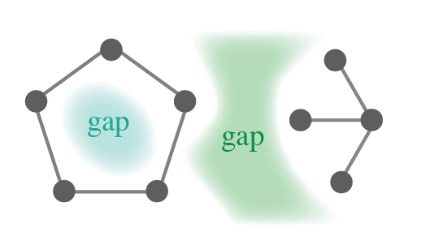
\includegraphics[scale=.4]{IGT.jpg}\end{center}
\end{frame}

%%%%%%%%%%%%%%%%%%%%%%%%%%%%%%%%%%%%%%%%%%%%%%%%%%%%%%%%%%%%%

\begin{frame}{IGT -- How to evaluate the gap}
	\begin{itemize}
	\item Characterize information gaps as topological cavities: dimension 0 means disconnected network components; dimension 1, known as 1-cycles, represent non-triangular loops of edges.
	\item \textbf{Humans create induced subgraphs with an increasing number of 1-dimensional cavities.}
	\item Reward based on IGT:
	\begin{equation}
    \mathcal{F}_{\text{IGT}}(S_t) = \beta_1(S_t),
    \end{equation}
    where $\beta_1(S_t)$ counts the number of topological gaps (1-dimensional cavities) in subgraph $S_t$.
    
	\end{itemize}
%\begin{center} 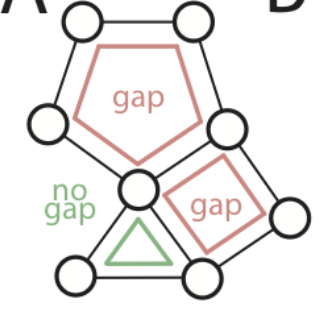
\includegraphics[scale=.4]{gap.png}\end{center}
\end{frame}


%%%%%%%%%%%%%%%%%%%%%%%%%%%%%%%%%%%%%%%%%%%%%%%%%%%%%%%%%%%%%

\begin{frame}{What drives curiosity? -- Compression Progress Theory}
	Curiosity is the drive to obtain information that improves the compression of a mental model and thereby lowers its cost of representation.\\
	Compression Progress Theory suggests curiosity drives us to compress information, improving understanding over time.
	
\begin{center} 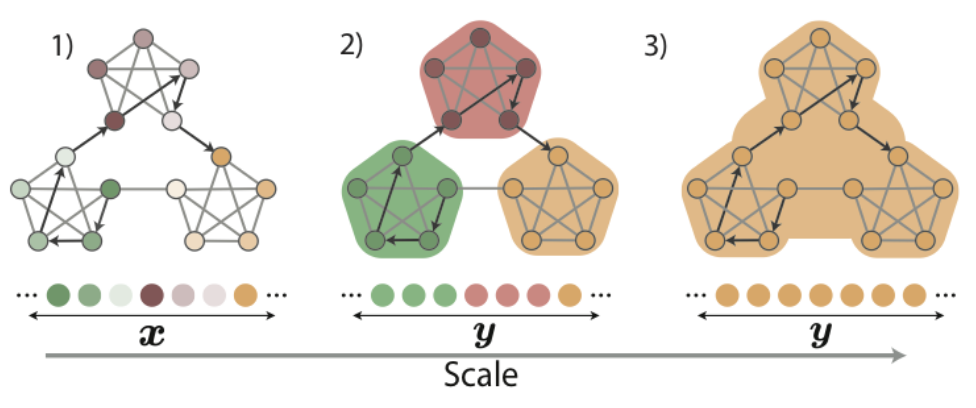
\includegraphics[scale=.5]{scale.png}\end{center}
\end{frame}
%%%%%%%%%%%%%%%%%%%%%%%%%%%%%%%%%%%%%%%%%%%%%%%%%%%%%%%%%%%%%
\begin{frame}
\begin{itemize}

    \item \textbf{Rate-Distortion Function:} Define scales of description by clustering nodes, then compute the information rate for each clustering. 
    \item \textbf{Network Compressibility:} The compressibility of the network is quantified as the average reduction in the information rate across all scales:
    \begin{equation}
    C = H - \frac{1}{t} \sum_{s} R(s),
    \end{equation}
    representing the maximal reduction in information rate from the original (uncompressed) network to the optimally compressed one.
    
   
\end{itemize}
\begin{center} 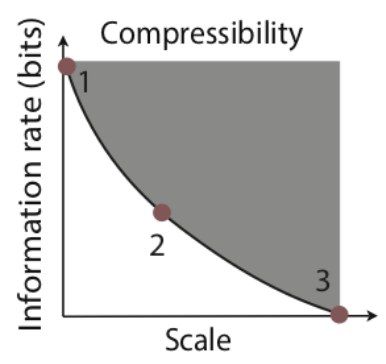
\includegraphics[scale=.45]{rate.png}\end{center}
\end{frame}
%%%%%%%%%%%%%%%%%%%%%%%%%%%%%%%%%%%%%%%%%%%%%%%%%%%%%%%%%%%%%
\begin{frame}
\frametitle{Compression Progress Theory (CPT)}
\begin{itemize}
    \item \textbf{Random Walk Entropy:} For a subgraph $S_t$, the entropy of a random walk on this graph is given by:
    \begin{equation}
    H = -\sum_{i} \pi_i \sum_{j} P_{ij} \log P_{ij},
    \end{equation}
    where $\pi_i$ is the stationary distribution, and $P_{ij}$ is the transition probability from node $i$ to node $j$.
\end{itemize}
\textbf{Reward of CPT}:
\begin{equation}
    \mathcal{F}_{\text{CPT}}(S_t) = H - \frac{1}{t} \sum_{s} R(s),
    \end{equation}
    where $H$ is the entropy of the unclustered random walk and $R(s)$ is the rate-distortion curve representing information rate as a function of scale $s$.

\end{frame}

%%%%%%%%%%%%%%%%%%%%%%%%%%%%%%%%%%%%%%%%%%%%%%%%%%%%%%%%%%%%%

\section{Reinforcement learning for graph exploration}
\begin{frame}
\frametitle{Reinforcement Learning for Graph Exploration}
\begin{itemize}
    \item Markov Decision Process setup for graph exploration:
    \begin{itemize}
        \item States: Subgraph induced by visited nodes, $S_t = G[V_t]$.
        \item Actions: Transition to a neighbor node, $A(S_t) = N(v_t) \setminus V_t$.
        \item Transition: Deterministic to the next state, $P(S_{t+1} | S_t, v) = 1$ if $v \in A(S_t)$.
        \item Reward: Defined by curiosity theories, $R_t = \mathcal{F}(S_t)$.
    \end{itemize}
    
    \item Policy and value function:
    \begin{equation}
    \pi = \arg \max_{v \in A(S_t)} Q(S_t, v), \quad Q(S_t, v) = \text{expected sum of future } R_t.
    \end{equation}
    
\end{itemize}
\end{frame}

%%%%%%%%%%%%%%%%%%%%%%%%%%%%%%%%%%%%%%%%%%%%%%%%%%%%%%%%%%%%%


\section{Curiosity-biased Node Centrality}
\begin{frame}
\frametitle{Curiosity-biased Node Centrality}
\textbf{From PageRank to Curiosity-biased Centrality:}
PageRank measures node importance by simulating a random walker on the network. A node's score increases with more incoming links or if linked by other important nodes.

\textbf{Adapting PageRank with Curiosity:}
\begin{itemize}
    \item \textbf{Traditional PageRank:} PageRank assigns centrality scores to nodes, represented by the stationary distribution $\eta$ of a Markovian random walk. With probability $\alpha$, a walker moves from node $v_i$ to a neighboring node $v_j$. Alternatively, with probability $1-\alpha$, the walker teleports to a random node in the network. The stationary distribution is given by:
\begin{equation}
(I - \alpha P_{ij}^t) \eta_i = (1 - \alpha)q_j.
\end{equation}

 \end{itemize}
\end{frame}

\begin{frame}
\frametitle{Curiosity-biased Node Centrality Derived from PageRank}

\textbf{Understanding Traditional PageRank:}
\begin{itemize}
    \item PageRank measures the importance of each node within a graph based on the number and quality of links to that node.
    \item It simulates a random walk: a surfer moves from one node to another through edges or jumps to a random node with probability $1-\alpha$, typically set around 0.85.
    \item The steady-state probability (stationary distribution $\eta$) of being on any given node reflects its 'centrality' or importance.
\end{itemize}
\end{frame}

 \begin{frame}
 \begin{itemize}
    \item Curiosity-biased PageRank adjusts this formula by incorporating a curiosity-driven weighting factor based on the concepts from Information Gap Theory (IGT) and Compression Progress Theory (CPT).
    \item For a non-Markovian walker at node $v_l$ with a path history $V_l = \{v_1, \dots, v_{l-1}, v_l\}$ and induced subgraph $S_l$, the new transition probability to node $v_m$ is:
\begin{equation}
P_{lm}^{F}(S_l) = 
\begin{cases} 
(1-p_g)\frac{1}{|A(S_l)|} + p_g \frac{(Q(S_l, v_m))^{-1}}{\sum_{n \in A(S_l)}(Q(S_l, v_n))^{-1}} & \text{if } v_m \in A(S_l), \\
0 & \text{otherwise}.
\end{cases}
\end{equation}
Here, $p_g \in [0, 1]$ controls the walk's greediness, and $Q(S_l, v_m)$ reflects the value of moving to node $v_m$ given the subgraph $S_l$.

\end{itemize}
\end{frame}


 \begin{frame}
\textbf{Curiosity-biased Transition Probabilities:}
\begin{itemize}
    \item Adjusted probabilities ($P_{lm}^{F}$) depend on the historical path and induced subgraph, making the walk history-dependent, contrary to the Markovian assumption of traditional PageRank.
    \item $p_g$ controls the balance between exploration (discovering new nodes) and exploitation (visiting nodes believed to offer valuable information).
    \item The transition modifications ensure that nodes leading to high curiosity rewards are more likely to be visited, reshaping the centrality landscape to highlight areas of potential interest.

\end{itemize}
\end{frame}


%%%%%%%%%%%%%%%%%%%%%%%%%%%%%%%%%%%%%%%%%%%%%%%%%%%%%%%%%%%%%

\begin{frame}
\frametitle{Methodology: Reinforcement Learning on Knowledge Graph}
\begin{enumerate}
    \item Learning model: based on interaction with the environment.
    \item Agent makes decisions to achieve a goal.
    \item Intrinsic motivation: driving exploration through curiosity;
    \item Applying network theories to guide exploration in graph environments:
    \begin{itemize}
    \item Information Gap Theory (IGT): Seeks to fill knowledge gaps.
    \item Compression Progress Theory (CPT): Aims for more efficient data encoding.
\end{itemize}
	\item Use Graph Neural Networks (GNN) for navigation tasks.
\end{enumerate}
\end{frame}
\begin{frame}{Reinforcement learning for graph exploration}

\begin{center} 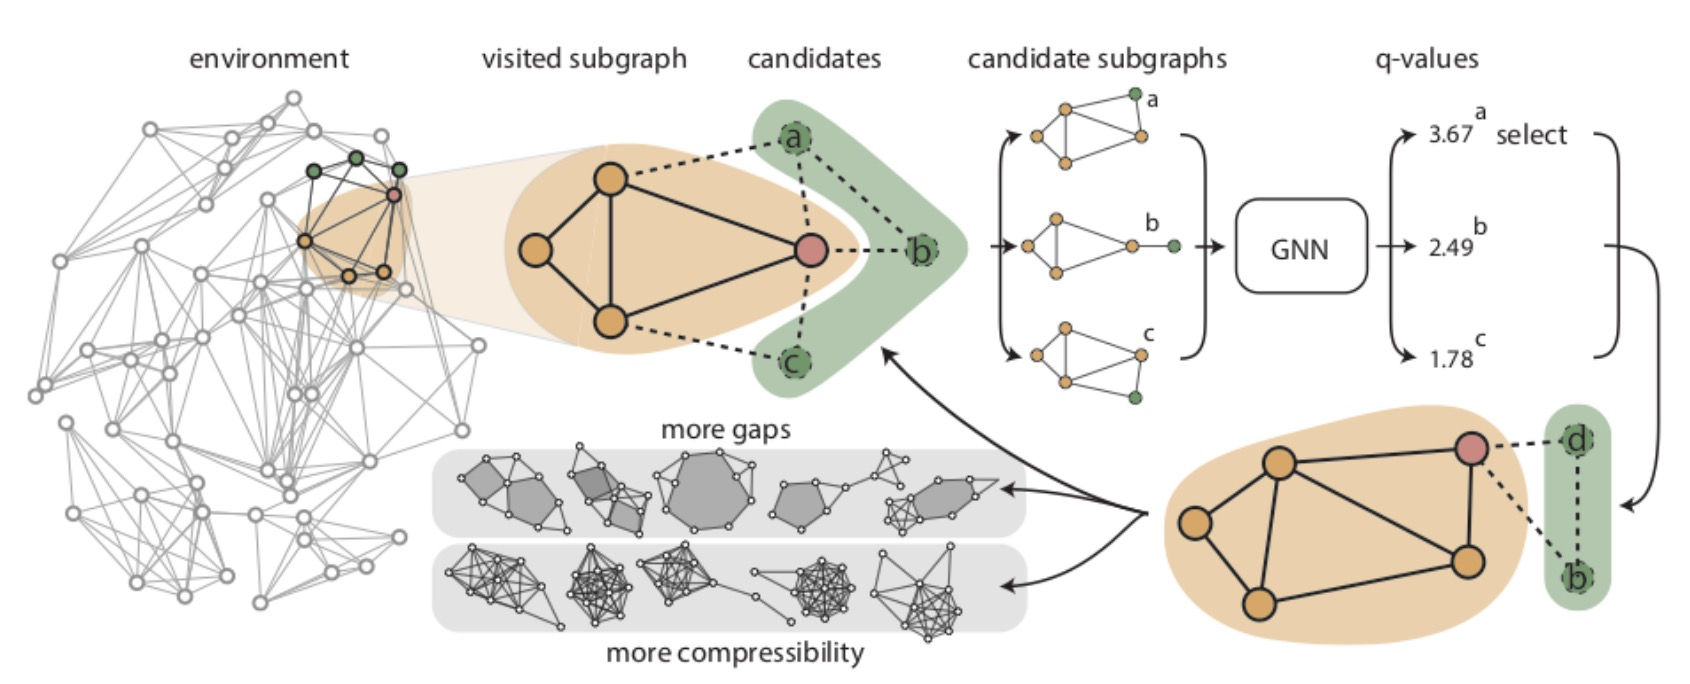
\includegraphics[scale=.4]{RL.jpg}\end{center}

\end{frame}


\section{Experiments}
\begin{frame}
\frametitle{Experiment 1: Exploration in Synthetically Generated Networks}
\textbf{Objective:} Assess how the curiosity-based models perform in different synthetic graph environments.

\textbf{Graph Models Used:}Random Geometric (RG), Watts-Strogatz (WS), Barabási-Albert (BA), Erdős-Rényi (ER)

\textbf{Methodology:}
\begin{itemize}
    \item 100 training environments, 10 validation, and 10 testing for each graph type, 50 nodes each, exploration episode lasts for 10 steps.
    \item Agents are evaluated against baselines: Random, Greedy, Max Degree, Min Degree.
\end{itemize}

\textbf{Evaluation Metrics:}Total average reward gathered by agents; performance comparison against baseline methods.

\end{frame}

\begin{frame}
\frametitle{Results and Discussion for Experiment 1}
\textbf{Key Findings:}
\begin{itemize}
    \item In Random Geometric and Watts-Strogatz networks, the curiosity-driven agents outperformed all baselines in terms of total average rewards.
    \item In Barabási-Albert networks, agents also performed well, highlighting the effectiveness of the curiosity models in scale-free environments.
    \item The Greedy method showed competitiveness but at a higher computational cost compared to our GNN agents.
\end{itemize}
\end{frame}

\begin{frame}
\frametitle{Experiment 2: Predicting Human Choices}
\textbf{Objective:} Evaluate the model's ability to predict human navigational choices in real-world graph environments.\\
\textbf{Datasets Used:} MovieLens, Amazon Books, Wikispeedia.\\
\textbf{Methodology:}
\begin{itemize}
    \item Represent user actions as graph explorations.
    \item Train GNN models using curiosity-based rewards.
\end{itemize}
\textbf{Evaluation Metrics:}
\begin{itemize}
    \item Performance of curiosity-driven models vs. standard PageRank in predicting user choices.
    \item Percentage improvement in predicting transitions made by humans using curiosity-biased.
\end{itemize}
\end{frame}

\begin{frame}
\frametitle{Results and Discussion for Experiment 2}
\textbf{Key Findings:}
\begin{itemize}
    \item Curiosity-driven models significantly improved the prediction of human choices across all three datasets, with the most notable improvement seen in the Wikispeedia dataset.
    \item Incorporating both IGT and CPT theories yielded the best results, particularly in navigating the Wikispeedia paths.
    \item The models also showed a notable improvement in the MovieLens and Amazon Books datasets, suggesting a broad applicability.
\end{itemize}
\end{frame}

\section{Results}
\begin{frame}
\frametitle{Results and Discussion}
\begin{itemize}
    \item Models show improved exploration capability.
    \item Curiosity-based methods better predict human decisions in graphs.
\end{itemize}
\end{frame}


\begin{frame}
\textbf{Discussion Points 1:}
\begin{itemize}
    \item The success in RG and WS networks suggests that the curiosity-driven models are particularly effective in navigating small-world and geometrically structured environments.
    \item The performance in BA networks indicates the model's adaptability to environments with heterogeneous connectivity.
    \item Efficiency of GNNs presents a significant advantage over traditional greedy approaches, particularly in larger or more complex graphs.
\end{itemize}
\end{frame}

\begin{frame}

\textbf{Discussion Points 2:}
\begin{itemize}
    \item The marked improvement in the Wikispeedia dataset highlights the potential of curiosity-driven models in goal-oriented navigation tasks.
    \item Success across diverse datasets indicates the robustness and versatility of curiosity-driven exploration strategies.
    \item The combination of IGT and CPT theories suggests that a multifaceted approach to modeling curiosity can yield significant benefits in real-world applications.
\end{itemize}
\end{frame}
\section{Conclusion}
\begin{frame}
%\frametitle{Conclusion}
\textbf{Key Takeaways:}
\begin{itemize}
    \item Demonstrated the efficacy of intrinsic motivation (curiosity) in enhancing graph exploration tasks.
    \item The incorporation of human-like curiosity models into reinforcement learning offers notable advantages over conventional methods, particularly in complex or less structured environments.
    \item Curiosity-driven models provide a promising avenue for predicting and understanding human behavior in information navigation tasks.
\end{itemize}
\end{frame}

\begin{frame}
\textbf{Future Work:}
\begin{itemize}
    \item Investigating other forms of intrinsic motivation and their impacts on exploration and learning.
    \item Application of curiosity-driven exploration strategies to other domains such as social networks, e-commerce, and educational platforms.
    \item Further refinement of models to improve computational efficiency and scalability.
\end{itemize}

\end{frame}

\begin{frame}
\frametitle{Questions?}
\textbf{Final Note:}
The integration of curiosity-driven approaches opens new paths for enhancing AI's understanding and navigation of complex, interconnected data structures, reflecting a more human-like approach to information discovery and learning.\\
Thank you for your attention! Any questions?
\end{frame}


%%%%%%%%%%%%%%%%%%%%%%%%%%%%%%%%%%%%%%%%%%%%%%%%%%%%%%%%%%%%%
\end{document}